\documentclass[11pt]{article}
\usepackage[margin=1in]{geometry}
\usepackage{amsmath,amssymb}
\usepackage{booktabs}
\usepackage{xcolor}
\usepackage{enumitem}
\usepackage{pgfplots}
\pgfplotsset{compat=1.17}
\usepackage[colorlinks=true,linkcolor=blue,urlcolor=blue]{hyperref}

\title{\textbf{Fine-Tuning a Code LLM to Generate Interactive\\
Geometry-Diagram Constructions}\\[4pt]
\large Dataset Construction, Method, and Results}
\author{Aditya Dhull}
\date{June 2026}

\begin{document}
\maketitle

\begin{abstract}
\noindent We fine-tune \textbf{Qwen2.5-Coder-14B-Instruct} to translate a
natural-language Olympiad geometry problem into an \emph{ordered GeoGebra
construction} (a JSON list of steps) that renders an interactive, draggable
diagram. Training uses \textbf{QLoRA} (4-bit base + low-rank adapters) on a
\textbf{292-problem} corpus that was assembled and verified by a custom
headless-GeoGebra pipeline: every construction renders, every stated claim is
numerically checked, every entity is consistently labelled
\texttt{final}/\texttt{construction}, and no dead steps remain. On
\textbf{39 held-out, unseen} problems the model produces \textbf{100\%}
parseable JSON and \textbf{85\%} render-valid figures, a $\sim$14-point
improvement over an earlier 14B run on the un-cleaned data (71\%).
\end{abstract}

\section{Problem and Task}
The system maps a problem statement (e.g.\ ``Let $ABC$ be a triangle with
incentre $I$; the incircle touches $BC$ at $D$\ldots'') to a JSON object
\texttt{\{"construction\_steps": [\,\ldots\,]\}}. Each step has a \texttt{name},
a \texttt{type} (\texttt{final} = shown, \texttt{construction} = hidden helper),
a \texttt{class} (point/line/segment/circle/\ldots), an optional \texttt{label},
and a \texttt{command} in native GeoGebra syntax that references earlier steps.
Steps must be in constructible order; free base points use coordinates and
everything else is derived (\texttt{Midpoint}, \texttt{Intersect},
\texttt{Circle}, \texttt{AngleBisector}, \texttt{Reflect}, \ldots). Because the
output is essentially \emph{code} with strict syntax and ordering constraints,
the task is well suited to a code-specialised LLM.

\section{Dataset Construction and Verification}
The corpus has three sources, all passed through the same verification gate.

\paragraph{(1) Gold seed --- 82 problems.} Hand-curated, hand-checked problems
that define the schema and quality bar.

\paragraph{(2) Generated --- 150 problems.} Authored in-session and gated by a
headless-GeoGebra validator plus machine-checkable semantic assertions
(collinear, concyclic, concurrent, tangent, Ptolemy, \ldots). They span classic
configurations: Miquel/Euler-line/nine-point/Feuerbach, Simson/Steiner,
Pascal/Pappus/Desargues/Monge, Ptolemy, power-of-a-point/Menelaus/Ceva,
symmedian/Lemoine, excentral/Nagel/Gergonne, Napoleon/Fermat, and quadrilateral
metric theorems.

\paragraph{(3) New --- 60 problems.} Generated in two rounds. Round~1 used
agents anchored on classic lemmas; a strict adversarial audit (below) kept only
$\sim$25\%, because most duplicated the existing 150 or carried logic defects.
Round~2 used four \emph{novel-territory} agents (special triangle centres;
circle/radical/inversion/pole--polar; concrete metric problems with numeric
answers; quadrilateral lemmas), each \emph{numerically self-verifying every
claim} before returning it --- yielding a far higher survival rate.

\paragraph{Verification gate.} Every candidate is checked for:
\begin{enumerate}[noitemsep,topsep=2pt]
  \item \textbf{Renderability} --- each step builds a real object across
  multiple random-parameter renders in a real (headless) GeoGebra engine.
  \item \textbf{Claim fidelity} --- full-precision coordinates are probed and
  the statement's assertion is tested numerically (collinearity, concyclicity,
  equal lengths, perpendicularity, ratios, concurrency, or an exact value).
  \item \textbf{Meaningful steps} --- no step is built and then left unused.
  \item \textbf{Visibility} --- every object named in the statement is
  \texttt{final}; pure scaffolding is \texttt{construction}.
  \item \textbf{Novelty} --- cross-dataset near-duplicate scan against all other
  problems.
\end{enumerate}

\begin{table}[h]
\centering
\begin{tabular}{lrr}
\toprule
Source & Problems & In training split \\
\midrule
Gold (hand-curated)      & 82  & 71 \\
Generated (verified)     & 150 & 130 \\
New (audited, 2 rounds)  & 60  & 52 \\
\midrule
\textbf{Total}           & \textbf{292} & \textbf{253} \\
\bottomrule
\end{tabular}
\caption{Final corpus. The held-out evaluation set is the remaining
$39$ problems ($11$ gold $+$ $20$ generated $+$ $8$ new), never seen in
training. The $253$ training problems are paraphrase-augmented to
$\mathbf{850}$ examples.}
\end{table}

\section{Base Model Selection}
We chose \textbf{Qwen2.5-Coder-14B-Instruct} (Apache-2.0). Rationale:
\begin{itemize}[noitemsep,topsep=2pt]
  \item \textbf{Code specialisation.} The target is GeoGebra command syntax;
  a top open \emph{code} model minimises command hallucination.
  \item \textbf{Size fit.} In 4-bit it is $\sim$9.3\,GB and fits a single
  16\,GB GPU (Kaggle T4/P100) with room for activations and adapters.
  \item \textbf{Right capacity for the data.} A 32B model was considered but
  rejected: it does not fit one 16\,GB GPU (needing fragile multi-GPU model
  parallelism) and is over-sized for a 292-problem LoRA task. 14B is the
  sweet spot.
  \item \textbf{Licensing \& cost.} Apache-2.0, trainable for free on Kaggle.
\end{itemize}

\section{Fine-Tuning Method}

\subsection{QLoRA and why 4-bit}
We use \textbf{QLoRA}: the pretrained base is loaded in \textbf{4-bit} (NF4,
double quantisation) and \emph{frozen}; only small \textbf{low-rank adapter}
matrices are trained (in higher precision). 4-bit quantisation is the enabling
choice:
\begin{table}[h]
\centering
\begin{tabular}{lrl}
\toprule
Precision & Base weights (14B) & Fits one 16\,GB T4? \\
\midrule
fp16 / bf16 (16-bit) & $\sim$28\,GB & No (out-of-memory) \\
int8 (8-bit)         & $\sim$14\,GB & Tight, little headroom \\
\textbf{nf4 (4-bit)} & $\mathbf{\sim 9.3}$\,\textbf{GB} & \textbf{Yes, with room} \\
\bottomrule
\end{tabular}
\caption{Why 4-bit: it shrinks the frozen base enough to leave VRAM for
activations and optimiser state, making single-GPU fine-tuning of a 14B model
feasible on free hardware. Quantisation error is absorbed by the trainable
adapters, so accuracy loss is negligible for this task.}
\end{table}

\noindent Only $\mathbf{137{,}625{,}600}$ parameters are trained
($\mathbf{0.92\%}$ of $14.9$B), so the saved artefact is a $\sim$550\,MB
adapter rather than a full checkpoint.

\subsection{Configuration}
Training used the Unsloth library (single GPU, paged 8-bit AdamW), with the loss
computed \emph{only on the assistant JSON} (prompt tokens masked).
\begin{table}[h]
\centering
\begin{tabular}{ll}
\toprule
Setting & Value \\
\midrule
Base model            & \texttt{Qwen2.5-Coder-14B-Instruct} (4-bit NF4) \\
Adapter (LoRA)        & $r=32$, $\alpha=32$, dropout $0$ \\
Target modules        & q,k,v,o,gate,up,down\_proj \\
Trainable params      & $137.6$M ($0.92\%$) \\
Batch / grad-accum    & $1 \times 8$ (effective batch $8$) \\
Epochs / steps        & $2$ / $214$ \\
Learning rate         & $2\times10^{-4}$, cosine, $5\%$ warmup \\
Max sequence length   & $1536$ \\
Optimiser             & \texttt{adamw\_8bit}; loss on responses only \\
Hardware              & 1$\times$ Kaggle GPU (T4/P100, 16\,GB) \\
Wall-clock            & $9871$\,s $\approx$ \textbf{2\,h\,44\,m} \\
\bottomrule
\end{tabular}
\caption{Fine-tuning configuration.}
\end{table}

\subsection{Training dynamics}
The loss decreased smoothly and monotonically with no instability.

\begin{center}
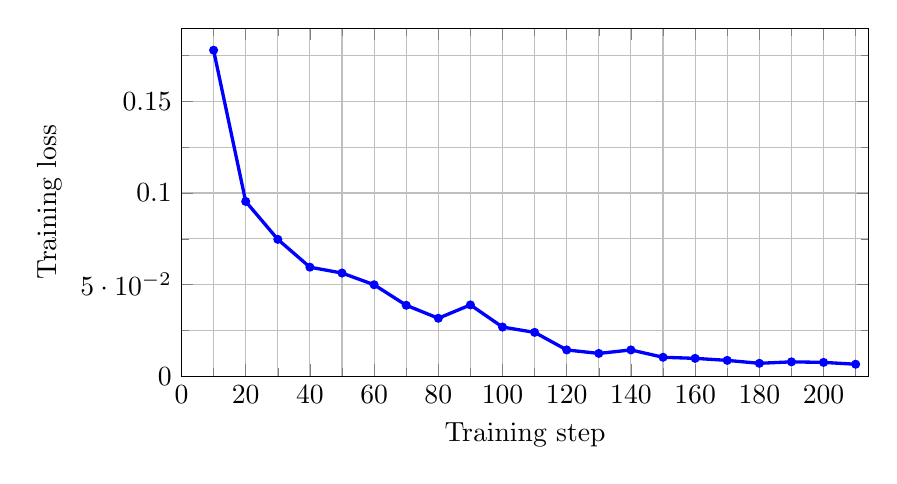
\begin{tikzpicture}
\begin{axis}[
  width=0.85\textwidth, height=6cm,
  xlabel={Training step}, ylabel={Training loss},
  xmin=0, xmax=214, ymin=0, ymax=0.19,
  grid=both, minor tick num=1,
  every axis plot/.append style={very thick},
]
\addplot[blue,mark=*,mark size=1pt] coordinates {
(10,0.178)(20,0.0954)(30,0.0747)(40,0.0595)(50,0.0563)(60,0.0499)
(70,0.0387)(80,0.0316)(90,0.0389)(100,0.0268)(110,0.0239)(120,0.0143)
(130,0.0124)(140,0.0143)(150,0.0103)(160,0.0097)(170,0.0086)(180,0.0070)
(190,0.0078)(200,0.0075)(210,0.0065)};
\end{axis}
\end{tikzpicture}
\end{center}
\noindent Final training loss $\approx 0.006$. Such a low value is expected when
learning exact construction syntax from paraphrase-augmented data; the honest
quality signal is therefore the held-out render rate (\S\ref{sec:results}).

\section{Inference and Post-Processing}
At inference the model is loaded as base$+$adapter (4-bit) and decoded greedily.
Three light, deterministic fixes are applied to the raw output:
\begin{enumerate}[noitemsep,topsep=2pt]
  \item lower-case the \texttt{class} field;
  \item reorder \texttt{AngleBisector(P,Q,R)} so the named vertex is the middle
  argument;
  \item the interactive renderer auto-corrects a collapsed \texttt{Intersect}
  index (when a new point lands on an existing one).
\end{enumerate}

\section{Results on 39 Held-Out Problems}
\label{sec:results}
The model was evaluated on the $39$ never-seen problems by generating a
construction for each and re-rendering it in headless GeoGebra. A prediction
counts as \emph{render-valid} only if every step builds across multiple random
renders; an unparsed prediction counts as a failure.

\begin{table}[h]
\centering
\begin{tabular}{lrr}
\toprule
Metric & This run (14B, cleaned 292-set) & Prior 14B (un-cleaned data) \\
\midrule
Parseable JSON & $39/39 = \mathbf{100\%}$ & $100\%$ \\
Render-valid   & $33/39 = \mathbf{85\%}$  & $71\%$ \\
\bottomrule
\end{tabular}
\caption{Held-out results. The cleaned, audited, visibility-labelled corpus
lifts render-validity by $\sim$14 points.}
\end{table}

\paragraph{Failure analysis.} All six failures are isolated geometry slips on
the hardest constructions --- none are JSON or formatting errors.
\begin{table}[h]
\centering
\begin{tabular}{cll}
\toprule
\# & Cause & Category \\
\midrule
1 & \texttt{Angle(A,B,C)} used where \texttt{AngleBisector} was needed & wrong command \\
2 & \texttt{Line(A,Xdoubleprime)} --- \texttt{Xdoubleprime} never defined & undefined reference \\
3 & cevian feet \texttt{Ap/Bp/Cp} not built / degenerate & undefined / degenerate \\
4 & two lines parallel for the chosen coords $\Rightarrow$ no intersection & degenerate config \\
5 & \texttt{Intersect(\ldots,2)} --- second intersection does not exist & invalid index \\
6 & long incircle/parallel chain with a bad intermediate & complex hallucination \\
\bottomrule
\end{tabular}
\caption{The six render failures. Several (wrong command, invalid index) are the
class a generate$\to$validate$\to$repair loop would recover, so usable quality is
slightly above the raw $85\%$.}
\end{table}

\section{Conclusion and Future Work}
A 14B code LLM, QLoRA-tuned on a small but rigorously verified 292-problem
corpus, generalises to unseen Olympiad geometry problems at \textbf{85\%}
render-validity. The decisive factors were (i) a verification pipeline that
guarantees every training target renders, matches its stated claim, and is
consistently labelled, and (ii) 4-bit QLoRA, which makes single-GPU fine-tuning
of a 14B model feasible on free hardware. The clearest next lever is a
\emph{generate$\to$validate$\to$repair} loop that feeds a failing step and its
GeoGebra error back to the model for one or two retries, which would recover
the command/index failures and push render-validity past $90\%$.

\end{document}
